\documentclass[article]{jdssv}

%% -- packages -----------------------------------------------------------------
\usepackage{thumbpdf,lmodern}
\usepackage{amsmath,amssymb}
\usepackage{booktabs}
\usepackage{bm}

\raggedbottom
\renewcommand{\topfraction}{0.9}\renewcommand{\bottomfraction}{0.8}\renewcommand{\textfraction}{0.07}
\renewcommand{\floatpagefraction}{0.7}\setcounter{topnumber}{2}\setcounter{totalnumber}{4}
\newcommand{\BC}{\textsf{BC}}
\newcommand{\FC}{\textsf{FC}}
\newcommand{\LV}{\textsf{LV}}
\newcommand{\OR}{\textsf{OR}}

%% -- metadata -----------------------------------------------------------------
\author{Jan Janou\v{s}ek\\Charles University
   \And Michal Pe\v{s}ta\\Charles University}
\Plainauthor{Jan Janousek, Michal Pesta}

\title{Decision Maps for the Basketball End Game: An Exact Game Estimated from 26 Seasons of Play-by-Play Data}
\Plaintitle{Decision Maps for the Basketball End Game: An Exact Game Estimated from 26 Seasons of Play-by-Play Data}
\Shorttitle{Decision Maps for the Basketball End Game}

\Abstract{
In the last seconds of a close basketball game, coaches make a handful of discrete choices that decide
games: foul or defend when leading by three, make or deliberately miss a final free throw when trailing,
spend a timeout to advance the ball. We build a reproducible pipeline that turns 26 seasons of public
National Basketball Association (NBA) play-by-play data (31{,}238 games, 2000-01 to 2025-26) into an exact
end-game model and into decision maps that show, for every tenth of a second, score and timeout state, the
choice that is optimal under the model, its win-probability margin and its sampling uncertainty, with observed coach behaviour drawn
on top. The model is a zero-sum stochastic game on a 0.1-second grid whose principal probabilities and durations
(rushed-shot curves by how a possession starts, rebound rates and dead-ball shares, foul, timeout and rebound times) are
estimated, and estimation and solution are bootstrapped by game. The solver is verified by an independent computation in exact
arithmetic, and a break-even rebound rate for the deliberate miss is derived in
closed form. Compared with a hand-set version of the same model, the estimated game removes most of the
value of fouling when up three with 3--5 seconds left (from $+11$ to $+14$ percentage points to between $-2.2$ and
$+2.1$, depending on how the trailing team inbounds), and makes the deliberate miss when down two worth 6.0 percentage
points with 2 seconds left and 5.1 with 5, a result that survives every sensitivity analysis we ran (each taken
separately) except assuming that a deliberate miss is rebounded no more often than an accidental one. The 2017-18 cap on late
timeouts is visible in the data to the season, and coaches used both deliberate strategies more often after it.
}

\Keywords{sports analytics, dynamic programming, stochastic game, decision visualisation, bootstrap, reproducibility}
\Plainkeywords{sports analytics, dynamic programming, stochastic game, decision visualisation, bootstrap, reproducibility}

\Address{
  Jan Janou\v{s}ek\\
  Department of Probability and Mathematical Statistics\\
  Faculty of Mathematics and Physics, Charles University\\
  Sokolovsk\'a 83, 186\,75 Prague 8, Czech Republic\\
  E-mail: \email{janousek@karlin.mff.cuni.cz}\\
  ORCID: \url{https://orcid.org/0009-0007-3731-4416}\\
\ \\
  Michal Pe\v{s}ta (corresponding author)\\
  Department of Probability and Mathematical Statistics\\
  Faculty of Mathematics and Physics, Charles University\\
  Sokolovsk\'a 83, 186\,75 Prague 8, Czech Republic\\
  E-mail: \email{pesta@karlin.mff.cuni.cz}\\
  ORCID: \url{https://orcid.org/0000-0001-5311-0797}
}

\begin{document}

%% ============================================================================
\section{Introduction} \label{sec:intro}

The last 24 seconds of a close basketball game are a small, rule-bound world. The score margin is a few
points, the clock is read to the tenth of a second, and the teams choose among a handful of actions: the
leading team can foul at once and send the opponent to the free-throw line instead of defending; the
trailing team can call a timeout, which in the last two minutes lets it inbound the ball in the frontcourt
(the \emph{advance}); a player shooting the last free throw while trailing can try to make it or miss it on
purpose and hope for an offensive rebound. Each of these choices has a literature, mostly built on
\emph{hand-set} models: win probabilities computed from league-average shooting percentages and assumed
rebound rates \citep{Annis2006, Kenter2015, SkinnerGoldman2015}, win-probability models that evaluate observed
decisions \citep{McFarlane2019}, empirical tests of strategic choices \citep{Secilmis2025}, or empirical decision
grids by clock state \citep{ZapataHall2024}. \citet{Annis2006} already compares fouling and defending when up three;
\citet{Kenter2015} already solves an alternating end-game recursion with empirically chosen inputs and draws optimal
actions over score and time; \citet{ZapataHall2024} makes a coloured decision grid a central output. What is new here
is not the decision map as such but the combination of a richer game whose principal inputs are estimated from
play-by-play data, timeouts and fouls to give in the state, sampling uncertainty propagated to signed action
margins, and observed behaviour drawn on the same axes. The hand-set model we compare with is our own
prototype with league-average inputs, not a reproduction of these papers.

Two things limit these analyses. First, the inputs that drive the answers are exactly the ones that are
hard to guess: how good is a three-point attempt that must be launched within four seconds of an inbound
pass, how often does a deliberately missed free throw come back to the shooting team, how much time does a
deliberate foul take. Second, the answer is a function of a multi-dimensional state (time, score,
possession, timeouts, team fouls) that tables of a few cells describe poorly, and point answers hide how
uncertain the inputs make them.

This paper is about the data-science pipeline and the graphics that address both problems. We
\begin{enumerate}
\item parse 26 seasons of public NBA play-by-play data into possession phases with the full end-game state,
      including timeouts left under the rules of each season and each team's foul to give (Section~\ref{sec:data});
\item write the end game as a zero-sum stochastic game \citep{Shapley1953} on a 0.1-second grid and solve it
      exactly by backward induction \citep{Bellman1957}, with a closed-form break-even condition for the
      deliberate miss that we verify symbolically (Section~\ref{sec:model});
\item estimate every probability and duration from the data, with a game-clustered bootstrap that re-estimates all inputs and
      re-solves the game in each replicate (Section~\ref{sec:estimation});
\item design \emph{decision maps}: small multiples of time-by-score strips that encode the optimal action and
      its win-probability margin in a diverging colour scale, mark where the bootstrap cannot sign the margin,
      and overlay observed coach behaviour before and after the 2017-18 rule change (Section~\ref{sec:maps}).
\end{enumerate}
The application (Section~\ref{sec:results}) revisits three questions: fouling when up three, the deliberate
free-throw miss, and the value of a timeout. Section~\ref{sec:checks} reports model checks and
reproducibility, and Section~\ref{sec:discussion} discusses limitations. The paper is in the tradition of
\citet{Romer2006}: an explicit model with inputs estimated from many seasons, compared with what decision
makers actually do. The 2017-18 cap on late timeouts, which \citet{Gibbs2022} cite as motivation for
studying timeouts, gives a natural before-and-after contrast for the observed behaviour.

%% ============================================================================
\section{Rules, data and possession phases} \label{sec:data}

\subsection{Rules that matter in the last 24 seconds}

Three rules of the official rule book \citep{nbarules} shape the end game. (i) In the last two minutes of the fourth period and of overtime, a team
that calls a timeout after the ball becomes dead may inbound it at the frontcourt line, saving the time
needed to bring it up the floor. (ii) Until a team reaches the penalty (its fifth team foul of a period, its fourth in
overtime, or its second in the last two minutes), a non-shooting foul gives the opponent only a side-out inbound, so a
team may have a \emph{foul to give}. (iii) From 2017-18 on, each team has seven timeouts per game, at most
four in the fourth period and at most two after its 3:00 mark; before, teams had six full timeouts and one
20-second timeout per half, with at most three full timeouts in the fourth period and two in its last two
minutes, and two full and one 20-second timeout in each overtime (in the data, three full timeouts in the
last two minutes occur in 30 of 40{,}978 team-games). The encoding follows the league's published rules and is
checked against the data, not a full audit of every season's rule book; the modern rule's reference to the
mandatory timeouts is not encoded. These rules are encoded in
the pipeline (function \code{timeouts_left()}), and the data confirm the 2017-18 change exactly
(Figure~\ref{fig:timeouts}a): the share of team-games with more than two timeouts in the last 3:00 of the
fourth period is 11--15\% in every season before 2017-18 and 0.2--0.8\% in every season since.

\subsection{Data}

We use the stats.nba.com play-by-play data for every regular-season game from 2000-01 to 2025-26 as
distributed by the \pkg{nba\_data} repository \citep{nbadata}: 26 seasons and 31{,}238 games. One source
covers all seasons, records the game clock to the tenth of a second in the last minute of each period, and
carries the official cumulative timeout counter and the team-foul count in the event text. A download
script fetches the 26 season files and records their checksums; a parser builds, for every event in the last
60 seconds of every period, the score, both teams' timeouts used (whole game, period, after 3:00) and both
teams' team fouls (period, last two minutes).

\subsection{Possession phases}

The unit of analysis is a \emph{possession phase}: the time from the moment a team gains the ball to its
first terminal action. A phase starts after the opponent's made field goal or made last free throw (a dead
ball inbounded in the backcourt, \BC), after a defensive rebound or a turnover (a live ball, \LV) or after an
offensive rebound (\OR); if the team calls a timeout before acting in the last two minutes, it continues as a
frontcourt inbound (\FC) from the time of the timeout. The phase ends at the first field-goal attempt,
turnover, defensive foul followed by free throws (a side-out is counted and the phase continues), or the end
of the period. Each phase stores its start type, the time left, the lead, the terminal action and its
time, both teams' timeouts left and foul to give, and the final result of the game. The last 60 seconds of
all periods give 677{,}135 phases. A rebound credited to a team rather than a player is a dead ball (the ball went
out of bounds), so its phase starts with an inbound, not live play; such phases are flagged. A separate table holds the last free throw of every two- or three-shot
trip in the last 60 seconds of the fourth period and overtime (46{,}995 trips), with the following rebound, the shooter's
leave-one-out season free-throw percentage and both teams' state.

Before 2006-07 the official counters show many more teams with all full timeouts used
(Figure~\ref{fig:timeouts}b, 2000-01 to 2005-06). We could not establish whether this reflects behaviour or a
different charging of mandatory timeouts, so timeout-dependent comparisons use 2006-07 to 2016-17 as the
earlier era; nothing else in the analysis depends on it.

%% ============================================================================
\section{The end-game model} \label{sec:model}

\subsection{State and moves}

Time is discretised into steps of $\Delta=0.1$ seconds and the horizon is 24 seconds. The shot clock is
therefore off, except after an offensive rebound with more than 14 seconds left, when it is reset to
14 seconds (the rule since 2018-19; the game encodes the current rules throughout). The rules then
distinguish two restarts \citep{nbarules}: a timeout leaves the shot clock as it was, so a live-ball timeout
after such a rebound leads to a frontcourt inbound with $14-c$ seconds on the shot clock (\textsf{FC14T};
13.4 seconds with the fitted timeout cost $c$), while a defensive foul in the frontcourt resets it to the larger of
14 seconds and the time left on it, so a side-out leads to a frontcourt inbound with 14 seconds (\textsf{FC14}). Let
$\kappa_s$ be the shot clock at the start of a phase of type $s$: 14 seconds for \OR\ and \textsf{FC14}, $14-c$ for
\textsf{FC14T}, and none for the other types. When $\kappa_s<t$ the offence must shoot within $\kappa_s$ seconds, and
holding the ball is a violation that gives the opponent a dead ball in the backcourt. A state is
$x=(t,d,s,a,b,g_a,g_b)$: time left $t$, lead $d$ of the team with the
ball, start type $s\in\{\BC,\FC,\LV,\OR,\textsf{FC14},\textsf{FC14T}\}$, timeouts left $a,b\in\{0,1,2^+\}$ of the offence and the defence,
and fouls to give $g_a,g_b\in\{0,1\}$. $V(x)$ is the probability that the team with the ball wins, with overtime
worth $\frac12$: $V(0,d,\cdot)=\tau(d)=\mathbf{1}\{d>0\}+\frac12\mathbf{1}\{d=0\}$. A bar, as in $\bar\cdot$,
denotes the remaining state components seen from the other team (timeouts and fouls to give swapped).
The defence commits to fouling or not at the start of a phase, and the foul then takes a fixed time. The moves are:

\begin{description}
\item[Defence.] At the start of a phase the defence may foul after $e_s$ seconds. With a foul to give
($g_b=1$) the foul is a side-out and the phase restarts; otherwise the offence shoots two free throws, or
three with probability $\pi_3$ when it trails by three or more
(the foul is ruled a shooting foul on a three-point attempt). With probability $\beta$ the offence beats a committed
foul: it may release its best shot before the foul arrives instead. Because a failed foul attempt looks like an
ordinary quick shot in play-by-play data, $\beta$ is not identified; the main analysis sets $\beta=0$ and
Section~\ref{sec:checks} uses 0.1, 0.2 and 1 (in up-three phases the offence shoots within the fitted foul time in
8--11\% of phases).
\item[Offence.] Before a \BC\ inbound, or $c$ seconds after gaining a live ball, the offence may call a
timeout and continue as \FC\ (as \textsf{FC14T} after an offensive rebound with more than 14 seconds left). Otherwise it holds the ball (worth $\tau(d)$) or attempts a $k$-point shot,
$k\in\{2,3\}$, after using $u\le t$ seconds. The attempt is made with probability $m_{k,s}(u)$, missed with
probability $\xi_{k,s}(u)$ (rebounded after $r$ seconds, by the offence with probability $\rho_{\mathrm{FG}}$, with
dead-ball shares $\theta_{\mathrm{FG}}$, $\eta_{\mathrm{FG}}$ as for free throws below),
drawn as a shooting foul with probability $p_{\mathrm{sf}}$ ($k$ free throws; the defence loses its foul to
give), lost as a turnover with probability $p_{\mathrm{to}}$, or not attempted at all with probability
$\nu_s(u)$ (the ball goes to the opponent).
\item[Free throws.] Each free throw is made with probability $q$. The shooter of the last free throw may miss
on purpose. A miss of type $j\in\{\mathrm{FT},\mathrm{DM}\}$ (ordinary, deliberate) is rebounded after $r'_j$ seconds, by the
shooting team with probability $\rho_j$. A share $\theta_j$ of these kept rebounds are team rebounds after the ball went
out of bounds off the defence, which restart with a frontcourt inbound (\FC, or \textsf{FC14} with more than 14
seconds left), and a share $\eta_j$ of the lost ones are team rebounds to the defence, which restart with the
opponent's backcourt inbound (\BC).
\end{description}

\subsection{Bellman equations}

Let $W(x)$ be the value after the defence has decided not to foul. With $U_k(x)$ the grid times
$0<u\le\min(t,\kappa_s)$ (for $k=2$ only those in a set $A_s$, Section~\ref{sec:estimation}) and $T(x)$ the timeout,
\begin{align}
W(x) &= \max\Big\{H(x),\; \max_{k,\,u\in U_k(x)} S_k(x,u),\; T(x)\Big\},\label{eq:W}\\
T(x) &= V(t-c,d,s_c,a-1,\cdot)\quad\text{if } s\in\{\LV,\OR\},\ a>0,\nonumber\\
S_k(x,u) &= \big(p_{\mathrm{to}}+\nu_s(u)\big)\big[1-V(t-u,-d,\LV,\bar\cdot)\big] + p_{\mathrm{sf}}\,F_k(t-u,d,a,b,g_a,0)\nonumber\\
 &\quad + m_{k,s}(u)\big[1-V(t-u,-(d+k),\BC,\bar\cdot)\big] + \xi_{k,s}(u)\,R(t-u-r,d),\nonumber\\
R(t',d) &= \rho_{\mathrm{FG}}K_{\mathrm{FG}}+(1-\rho_{\mathrm{FG}})\Lambda_{\mathrm{FG}}\quad\text{(kept and lost values at $t'$, defined below \eqref{eq:V})},\nonumber
\end{align}
the timeout term being absent otherwise; every value at a non-positive time is replaced by the terminal value, except that free throws awarded
at the buzzer are still shot ($F_k(0,\cdot)$). The hold value is $H(x)=\tau(d)$ if $t\le\kappa_s$ and
$H(x)=1-V(t-\kappa_s,-d,\BC,\bar\cdot)$ (a shot-clock violation) otherwise; the timeout leads to $s_c=\textsf{FC14T}$ if $s=\OR$
and $t>14$, else to $s_c=\FC$; \textsf{FC14} and \textsf{FC14T} use the \FC\ shot curves and foul time; durations are rounded to the grid; leads are clipped at $\pm12$. The defence's
foul is available only if it can be committed before the end ($t>e_s$); otherwise the foul branch is dropped
from \eqref{eq:V} (the timeout option of a \BC\ state remains). The defence's foul value is
$\Phi(x)=V(t-e_s,d,s',a,b,g_a,0)$ if $g_b=1$ (a side-out: $s'=\FC$ after \FC; after \OR, \textsf{FC14} or
\textsf{FC14T}, $s'=\textsf{FC14}$ if $t-e_s>14$ and \FC\ otherwise; $s'=\BC$ after \BC\ or \LV) and
$\Phi(x)=(1-\pi_3\mathbf{1}\{d\le-3\})F_2(t-e_s,d,\cdot)+\pi_3\mathbf{1}\{d\le-3\}F_3(t-e_s,d,\cdot)$ otherwise. With
$\Phi_\beta(x)=(1-\beta)\Phi(x)+\beta\max\{\Phi(x),\max_{k,\,u<e_s}S_k(x,u)\}$ (the offence may beat the foul),
\begin{equation}
V(x)=\begin{cases}\max\big\{\min\{W(x),\Phi_\beta(x)\},\,V(t,d,\FC,a-1,\cdot)\big\}, & s=\BC,\ a>0,\\
\min\{W(x),\Phi_\beta(x)\}, & \text{otherwise.}\end{cases} \label{eq:V}
\end{equation}
For free throws, with $M=1-V(t,-(d+1),\BC,\bar\cdot)$ the value after a make and, for a miss of type $j$ with
$t_j=t-r'_j$ (for a field goal, $t_{\mathrm{FG}}=t'$), $K_j=(1-\theta_j)V(t_j,d,\OR,\cdot)+\theta_jV(t_j,d,s_j,\cdot)$ after a kept rebound ($s_j=\textsf{FC14}$ if
$t_j>14$, else \FC) and $\Lambda_j=(1-\eta_j)[1-V(t_j,-d,\LV,\bar\cdot)]+\eta_j[1-V(t_j,-d,\BC,\bar\cdot)]$ after a lost one,
\begin{align}
F_1 &= \max\big\{\underbrace{qM+(1-q)\big[\rho_{\mathrm{FT}}K_{\mathrm{FT}}+(1-\rho_{\mathrm{FT}})\Lambda_{\mathrm{FT}}\big]}_{\text{try to make}},\nonumber\\
&\qquad \underbrace{\rho_{\mathrm{DM}}K_{\mathrm{DM}}+(1-\rho_{\mathrm{DM}})\Lambda_{\mathrm{DM}}}_{\text{miss on purpose}}\big\}, \label{eq:F}\\
F_j(t,d,\cdot) &= q\,F_{j-1}(t,d+1,\cdot)+(1-q)\,F_{j-1}(t,d,\cdot),\qquad j=2,3.\nonumber
\end{align}
Every transition either reduces $t$ or moves to a state whose value at the same $t$ is already known
(a free-throw trip reads the opponent's \BC\ value; a \BC\ timeout reads the \FC\ value), so the game is
solved exactly in one backward pass. The solver (\code{solve()} in \code{dp.py}) is compiled with
\pkg{Numba} \citep{numba}; it solves all $241\times 25\times 6\times 3^2\times 2^2$ states, with up to 240
shot timings each, in about one second.

\subsection{A break-even rebound rate for the deliberate miss}

The free-throw decision in \eqref{eq:F} has a closed form. Subtracting the two branches,
\begin{equation}
\text{miss} - \text{make} = (K_{\mathrm{DM}}-\Lambda_{\mathrm{DM}})\,\big(\rho_{\mathrm{DM}}-\rho^{\ast}\big),\quad
\rho^{\ast}=\frac{q\,(M-\Lambda_{\mathrm{DM}})+(1-q)\,\Delta}{K_{\mathrm{DM}}-\Lambda_{\mathrm{DM}}}, \label{eq:rstar}
\end{equation}
where $\Delta=\rho_{\mathrm{FT}}(K_{\mathrm{FT}}-\Lambda_{\mathrm{DM}})+(1-\rho_{\mathrm{FT}})(\Lambda_{\mathrm{FT}}-\Lambda_{\mathrm{DM}})$ is
what an ordinary miss is worth over a lost deliberate one. So whenever a kept deliberate miss is worth more than a lost one ($K_{\mathrm{DM}}>\Lambda_{\mathrm{DM}}$), missing on purpose is
optimal exactly when the deliberate-miss rebound rate exceeds $\rho^{\ast}$; with equal kept values $K$ and equal lost
values $\Lambda$ for both miss types it reduces to $\rho^{\ast}=(1-q)\rho_{\mathrm{FT}}+q(M-\Lambda)/(K-\Lambda)$. The break-even rate depends on
the state only through win probabilities that the solver already computes, so it can be drawn as a
curve against time and compared with other rebound rates (Figure~\ref{fig:breakeven}). The comparison is local:
it holds the continuation values $M$, $K_j$ and $\Lambda_j$ fixed, although these depend weakly on the rebound rate
through later free throws, so it is not a fully re-solved sensitivity analysis. The
identity was verified symbolically in \proglang{Mathematica} \citep{mathematica} (Appendix~\ref{app:check}).

%% ============================================================================
\section{Estimating the inputs} \label{sec:estimation}

\subsection{Rushed-shot curves}

The key inputs are $m_{k,s}(u)$: the probability of a made $k$-point shot when the team uses $u$ seconds from
a start of type $s$. The data show the time \emph{available} at the start of a play, not the time a team chose
to use; we identify the two by assuming that a team that chooses to shoot after $u$ seconds gets the same
quality of shot as a team that has only $u$ seconds. This is the usual assumption in end-game models, but it
is an identification assumption, not a fact: the sample also contains plays that end before the buzzer, shot
types are chosen, and excluding plays ended by a defensive foul selects possessions. The recommendations below
are conditional on it; Section~\ref{sec:checks} checks it directly. We estimate them from phases that start with at most 24 seconds left, where the time
available constrains the shot. Two samples contribute: every such phase in the first three periods, where
the last shot of a quarter is not driven by the score (157{,}502 phases), and fourth-period and overtime
phases of a team that is tied or trails by 1--3 and must score (13{,}990 phases, the \emph{pressure} sample).
Phases ended by a non-shooting defensive foul are excluded, because the curves describe what the offence gets
when the defence lets it play, and so are phases that start with a team rebound, because \OR\ and \LV\ are live
restarts in the game (dead-ball rebounds are modelled separately, Section~\ref{sec:model}): they are 44\% of
offensive-rebound starts after missed field goals in the unfiltered sample and 6\% of defensive ones. For each start type we fit three logistic regressions in $\log a$, where $a$
is the time available at the start of the play: the probability that a shot is attempted, and the success
rates of two- and three-point attempts. The effect of $\log a$ is a natural cubic regression spline with four
degrees of freedom \citep{Wood2017}, centred so that it is identifiable with the intercept, and the pressure
sample enters through an additive shift. The game uses the pressure versions,
$m_{k,s}(u)=P(\text{attempt}\mid u,s)\,P(\text{made}\mid k,u,s)$, and caps the attempt probability at
$1-p_{\mathrm{sf}}-p_{\mathrm{to}}$ so that the outcome probabilities sum to one.

Rare two-point attempts at the buzzer after a backcourt inbound are selected (a stolen inbound pass, a
long lob) and would overstate the value of a planned two. A two is therefore available to the offence only
where a fourth logistic regression of the same form puts the two-point share of attempts in the score-neutral
sample at a quarter or more (an empirical restriction, not a physical impossibility): from 4.1 seconds after
a backcourt inbound, 2.7 seconds after a live ball, and always after a frontcourt inbound or an offensive
rebound.

\begin{figure}[tbp]
\centering
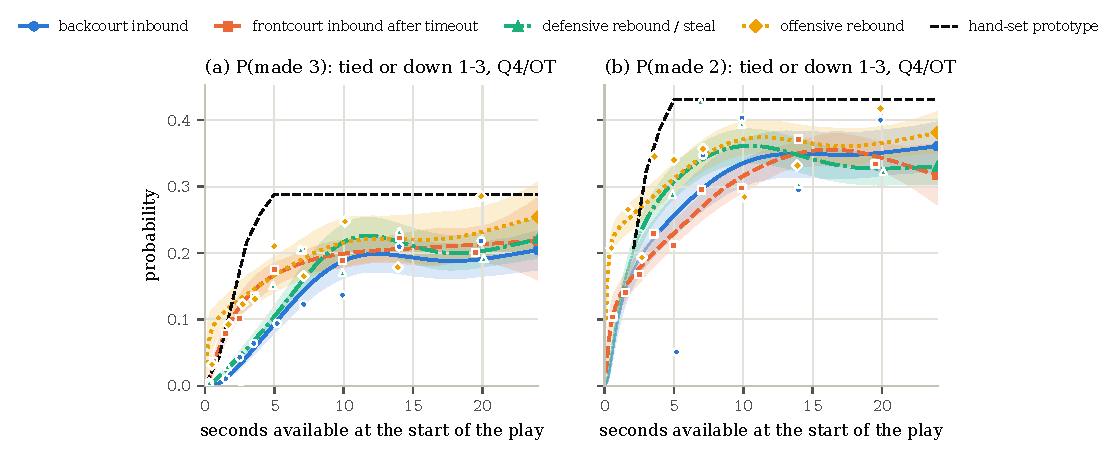
\includegraphics[width=\textwidth]{../figures/fig2_rushed_curves.pdf}
\caption{Rushed-shot curves: probability that a team tied or trailing by 1--3 in the fourth period or
overtime makes a three (a) or a two (b), by the seconds available at the start of the play and by how the
play starts. Lines: spline logits; bands: 90\% game-clustered bootstrap intervals; markers: binned data (shape by
start type);
dashed: the hand-set curve of the comparison model; faint thin lines in (b): durations at which the solver does not
allow a two. Each curve is the probability of an attempt times the success rate of a $k$-point attempt.}
\label{fig:curves}
\end{figure}

Figure~\ref{fig:curves} shows the result. From a backcourt inbound a team that must score makes a three with
probability 0.069 (90\% bootstrap interval 0.058--0.079) when it has 4 seconds and 0.161 (0.138--0.182) when it
has 8; after a timeout and a frontcourt inbound it makes one with probability 0.103 (0.087--0.119) with only 2
seconds. Above about 6 seconds the start type hardly matters, and the plateau of about 0.20 is well below the
league three-point percentage that hand-set models use. Frontcourt phases occur only in the fourth period and
overtime, so their curves have no score-neutral counterpart and no pressure shift.

\subsection{Scalar inputs}

Table~\ref{tab:inputs} lists the other inputs. The deliberate-miss rebound rate is estimated from last free
throws missed by a team trailing by 2 or 3 with at most 3 seconds left, a situation in which about three
quarters of last free throws are missed against an expected one in five. Rebounds logged after the buzzer, which
are credited arbitrarily, are excluded, and so are shooters without a season free-throw percentage (121 misses
remain; Appendix~\ref{app:figs} audits the event linkage). Of the kept rebounds, $\theta_{\mathrm{DM}}=0.23$ are team rebounds
(0.17 after ordinary misses), which the game treats as frontcourt inbounds (counting live rebounds only gives
$\rho_{\mathrm{DM}}=0.34$); of the lost ones, $\eta_{\mathrm{DM}}=0.32$ are team rebounds to the opponent (0.04 after
ordinary misses), which it treats as the opponent's backcourt inbound. Deliberate misses are rebounded sooner than
ordinary ones (0.69 against 1.08 seconds), and each miss type keeps its own delay; part of this gap is selection by
the clock, because a proxy miss with at most 3 seconds left must be rebounded before the buzzer to be retained,
whereas ordinary misses (at least 8 seconds left) are not so selected (Section~\ref{sec:checks} uses both delay
distributions). The rate is 0.49 (0.39--0.62) down two and 0.29 (0.14--0.43) down three. Whether leaders miss on purpose cannot be checked: leading by one with at most 3 seconds left, 32\% of last
free throws are missed against 21\% expected, too few deliberate misses to estimate a rate, so the maps apply the
trailing teams' rate to leaders as an extrapolation. Some misses in this proxy sample are
accidental. Suppose that shooters miss accidentally at their season rate whatever their intent, that the excess
misses are deliberate, and that accidental misses here are rebounded at the ordinary rate. Then the deliberate
share of the misses is $w=0.71$, the raw rate is $w\rho_{\mathrm{DM}}+(1-w)\rho_{\mathrm{FT}}$ and therefore a
\emph{lower bound} for $\rho_{\mathrm{DM}}$, and solving for $\rho_{\mathrm{DM}}$ gives the mixture-corrected rate
0.554 (0.433--0.691). The main analysis uses the raw rate, estimated at most 3 seconds before the end and
transported to longer times. Figure~\ref{fig:sens}a shows both by time window: the corrected rate is about 0.5 in
every window up to 8 seconds, which is compatible with a latent rate that does not depend on the time left
(although the interval for 5--8 seconds is wide); the raw rate falls (0.35 at 3--5 seconds, 0.31 at 5--8) because
fewer of those misses are deliberate. The sensitivity variants at 0.35 and 0.29 bracket these window-specific raw
rates. The ordinary rate uses misses with at least 8
seconds left (7{,}665). Durations are clipped (field-goal rebound and timeout times at 5
seconds, free-throw rebound times at 3, foul times at 6) before averaging. The foul times are measured from the start
of the phase (or from the offence's timeout) to the first non-shooting foul or side-out in fourth-period and overtime
phases with a non-zero lead; $\pi_3$ comes from fouls committed within 2 seconds of the start of a phase of a team
trailing by three; $p_{\mathrm{sf}}$ and $p_{\mathrm{to}}$ from pressure phases with at least 3 seconds available;
$\rho_{\mathrm{FG}}$, $\theta_{\mathrm{FG}}$ and $\eta_{\mathrm{FG}}$ from fourth-period and overtime misses with more than
1 second left.

\begin{table}[t]
\centering
\caption{Scalar inputs: hand-set values of the comparison model and estimates with 95\% game-clustered
bootstrap intervals ($B=1{,}000$).}
\label{tab:inputs}
\small
\begin{tabular}{lcc}
\toprule
Input & Hand-set & Estimate (95\% interval)\\
\midrule
Off.\ rebound, deliberate free-throw miss, $\rho_{\mathrm{DM}}$ (raw) & 0.13 & 0.438 (0.350, 0.531)\\
\quad mixture-corrected (sensitivity analysis) & -- & 0.554 (0.433, 0.691)\\
Off.\ rebound, ordinary free-throw miss, $\rho_{\mathrm{FT}}$ & 0.13 & 0.153 (0.145, 0.161)\\
Team rebounds among kept misses, deliberate, $\theta_{\mathrm{DM}}$ & 0 & 0.226 (0.123, 0.339)\\
\quad ordinary, $\theta_{\mathrm{FT}}$ & 0 & 0.169 (0.147, 0.190)\\
Team rebounds among lost misses, deliberate, $\eta_{\mathrm{DM}}$ & 0 & 0.324 (0.212, 0.442)\\
\quad ordinary, $\eta_{\mathrm{FT}}$ & 0 & 0.038 (0.033, 0.043)\\
Off.\ rebound, missed field goal (late), $\rho_{\mathrm{FG}}$ & 0.25 & 0.341 (0.334, 0.349)\\
\quad team rebounds among kept misses, $\theta_{\mathrm{FG}}$ & 0 & 0.209 (0.198, 0.220)\\
\quad team rebounds among lost misses, $\eta_{\mathrm{FG}}$ & 0 & 0.095 (0.090, 0.100)\\
Intentional foul ruled a three-shot foul, $\pi_3$ & 0.05 & 0.081 (0.056, 0.110)\\
Shooting foul per play, $p_{\mathrm{sf}}$ & 0.08 & 0.066 (0.061, 0.071)\\
Turnover per play, $p_{\mathrm{to}}$ & 0.13 & 0.089 (0.083, 0.094)\\
Free-throw percentage of late shooters, $q$ & 0.78 & 0.797 (0.796, 0.798)\\
Time to foul after a \BC\ start, $e_{\BC}$ (s) & 2.0 & 2.06 (2.02, 2.10)\\
\quad after an \FC\ start, $e_{\FC}$ (s) & 2.0 & 1.68 (1.64, 1.73)\\
\quad after an \LV\ start, $e_{\LV}$ (s) & 2.0 & 1.33 (1.29, 1.36)\\
\quad after an \OR\ start, $e_{\OR}$ (s) & 2.0 & 1.36 (1.25, 1.46)\\
Time to call a timeout from a live ball, $c$ (s) & -- & 0.59 (0.56, 0.63)\\
Rebound time after a missed field goal, $r$ (s) & 1.0 & 1.67 (1.66, 1.69)\\
Rebound time, deliberate free-throw miss, $r'_{\mathrm{DM}}$ (s) & 1.0 & 0.69 (0.56, 0.81)\\
\quad ordinary miss, $r'_{\mathrm{FT}}$ (s) & 1.0 & 1.08 (1.07, 1.11)\\
\bottomrule
\end{tabular}
\end{table}

\subsection{Uncertainty}

Uncertainty is propagated by a game-clustered bootstrap with Poisson weights \citep{EfronTibshirani1993,
OwenEckles2012}: each replicate draws an independent Poisson(1) weight for each game, re-fits every curve and
scalar input with these weights, re-solves the game and stores all map summaries. The shooters' season
free-throw percentages, which enter through $q$, the deliberate share $w$ and the expected miss rates of the
overlays, are computed once and held fixed. Replicates
are seeded by their index, so any replicate can be recomputed alone. We use $B=1{,}000$ replicates and report
pointwise 5--95\% percentile bands for curves and map quantities and 95\% intervals for scalar inputs. The
bands are not simultaneous, and the
share of replicates in which an action is better (counted among replicates in which the action is available) is
a bootstrap frequency, not a posterior probability. All these intervals describe the sampling variability of the estimated
inputs given the model; they do not cover misspecification of the game itself, which
Section~\ref{sec:checks} addresses through calibration.

%% ============================================================================
\section{Decision maps} \label{sec:maps}

A decision in the end game is a function of at least four variables (time, score, possession type,
timeouts), and its consequence is a signed number: how much win probability the better action adds. A
decision map shows this function as small multiples of \emph{heat strips}. Within a panel, each row is a
score margin and the horizontal axis is time left, on the solver's 0.1-second grid; panels vary the
discrete state (how the possession starts, timeouts, foul to give). The design follows four rules.

\begin{enumerate}
\item \emph{One signed quantity in a diverging scale.} The colour is the win-probability margin of one action
over the other in percentage points, on a two-hue diverging scale (blue for the action named in the
caption, red for the alternative) with a neutral grey at indifference and symmetric limits, so that the
colour reads as both the decision and its size \citep{Crameri2020, Wilke2019}.
\item \emph{Uncertainty as texture, not as a second colour.} Where the pointwise 90\% bootstrap band of the
margin (its 5th and 95th percentiles) includes zero, the strip is hatched; a band of exactly zero is a tie and is
left unhatched in neutral grey. This is a pointwise statement about sampling variability under the model and
needs no second colour legend.
\item \emph{Behaviour on the same axes.} Observed coach behaviour is drawn as dots whose area is proportional
to the share of teams taking the action (for the free throw, the excess over the rate expected from free-throw
percentages; open markers mark a deficit), circles for 2006-07 to 2016-17 and squares for 2017-18 to 2025-26,
placed in the strip of their score margin and matched to the panel's state as far as the data allow (the
captions state what is pooled). All overlays use seasons from 2006-07 on, omit sparse cells, and are descriptive:
phases in which a coach acted are not comparable to phases in which the coach did not.
\item \emph{Redundant encodings.} The preferred action is written inside the strip (``foul''\slash``defend'',
``miss''\slash``make'', or $+$\slash$-$ on shorter runs), so the sign does not depend on hue and the maps survive greyscale
printing (both arms of the scale darken with size); a black line marks sign changes between margins above 0.25
points; line styles separate the curves; the colour scale saturates (arrows on the colour bar); grey cells mark an
unavailable action. The categorical colours and the diverging pair were checked
with a colour-vision-deficiency validator, and the maps were inspected in greyscale at print size.
\end{enumerate}
The maps are generated from the solver's output arrays by \code{figures.py}.

%% ============================================================================
\section{Application: three end-game decisions} \label{sec:results}

\subsection{Foul or defend when leading by three}

Figure~\ref{fig:foulmap} is the decision map for the leading team. Without a foul to give and from a
backcourt inbound, fouling up one is never optimal (it costs 7--67 percentage points), and up two it costs up to 23
points and gains at most 0.3. With a foul to give, the side-out uses time without free throws, and it can pay even up one or two (up to
21 and 7 percentage points at 4--5 seconds; panel c). Leading by three, the answer depends on how the trailing
team gets the ball. When it must inbound in the backcourt without a timeout (panel a), fouling costs up to 2.8
percentage points (1.4 at 3 seconds, band 0.5 to 3.1; 1.6 at 5), and the 90\% band includes zero only from about 6
to 13 seconds. When the trailer has advanced the ball with a timeout (panel b), fouling at once gains 1.8 percentage
points with 3 seconds left (band 0.3 to 3.1), 1.5 with 5 (band $-0.2$ to 3.0) and at most 5.6 at 2.4 seconds, and
turns negative beyond about 10 seconds. Letting the offence beat the foul does not change the gain at 3 seconds even
with $\beta=1$, because within this timing model a shot released inside the 1.7-second foul time is worth less to the
trailer than being fouled. With a foul to give (panel c) fouling up three gains up to 4.3 percentage points, at
about 5 seconds.

\begin{figure}[tbp]
\centering
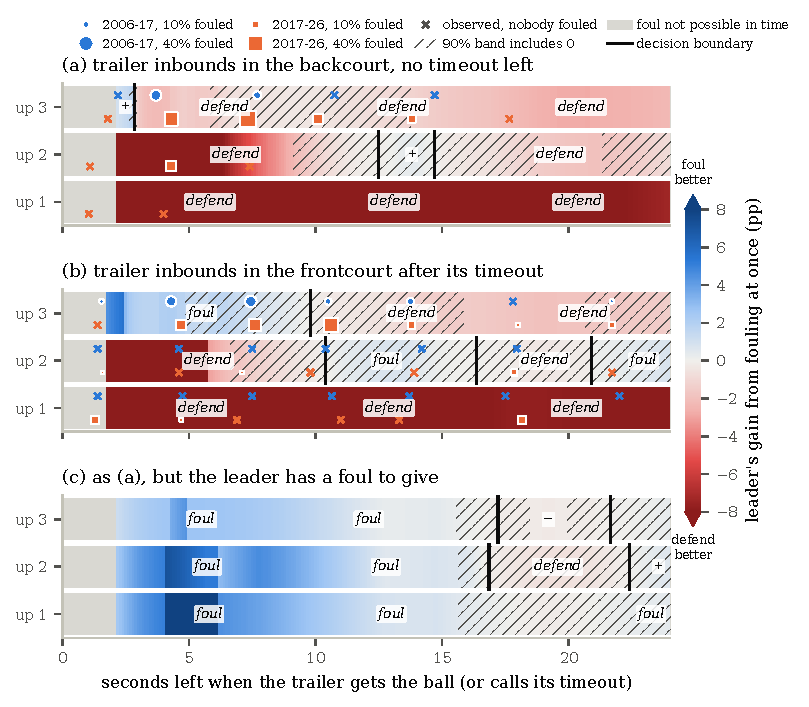
\includegraphics[width=\textwidth]{../figures/fig4_foul_map.pdf}
\caption{Decision map for the leading team: win-probability gain (percentage points) from fouling at once
instead of defending, by seconds left and lead; the trailer has no timeout left (in b, after its last) and no
foul to give, and the leader has no timeout and, in (a) and (b), no foul to give. Blue and the word ``foul''
(or $+$ on runs shorter than 1.5 seconds): foul; red and ``defend'' (or $-$): defend; hatched: the pointwise 90\% bootstrap band (5th--95th percentile) of the gain
includes zero. Black lines: decision boundary (a change of sign between margins
above 0.25 points); grey: the foul cannot be committed in time; the colour scale saturates at $\pm 8$. Markers
(area proportional to the share): phases in which a leader without a foul to give fouled deliberately (within 3
seconds of the decision point), after a dead-ball backcourt inbound of a trailer with no timeout left (a) or
after the trailer's last timeout (b), pooled over the leader's timeouts; circles 2006-07 to 2016-17 (blue),
squares 2017-18 to 2025-26 (orange); crosses: observed, nobody fouled; no marker: fewer than 10 phases (counts per
cell in \texttt{results/obs\_foul.csv}).}
\label{fig:foulmap}
\end{figure}

The dots show what coaches did. Between 3 and 12 seconds, leaders up three without a foul to give fouled
deliberately in 10.9\% of backcourt phases of a trailer with no timeout in 2006-07 to 2016-17 ($n=46$) and in
29.6\% from 2017-18 ($n=135$); after the trailer's last timeout the shares are 14.9\% ($n=201$) and 22.6\%
($n=217$). From a backcourt inbound at leads of one or two, where the map says never to foul, the rate is
0--1.6\%. In the capped era coaches fouled up three more often in both states, which the map rates as close to
indifference (margins between about $-2$ and $+3$ percentage points).

\subsection{Make or miss the last free throw}

Figure~\ref{fig:ftmap} is the decision map for the shooter of the last free throw. Trailing by two, the
deliberate miss gains 6.0 percentage points with 2 seconds left (band 4.8 to 7.3) and 5.1 with 5 when the
shooting team has no timeout, and 2.4 with 5 when it has one. The gain stays above one point up to 9.7 seconds
without a timeout and 6.8 seconds with one, and is positive up to about 11 seconds. The rebound rate is estimated
at most 3 seconds before the end and transported to longer times; beyond 8 seconds even the corrected rate is
unchecked (dotted lines). Trailing by one, a make ties the game and missing is
very costly. Leading by one with at most 3.3 seconds left, the shooter gains by missing (2.2 percentage points
at 2 seconds, 2.6 at 3, 0.4 at 1): the shooting team rebounds 44\% of deliberate misses, which usually ends the game, while a make hands
the opponent a possession. This rate comes from trailing shooters and is extrapolated to leaders
(Section~\ref{sec:estimation}), so the leading rows rest on an untested transfer.

\begin{figure}[tbp]
\centering
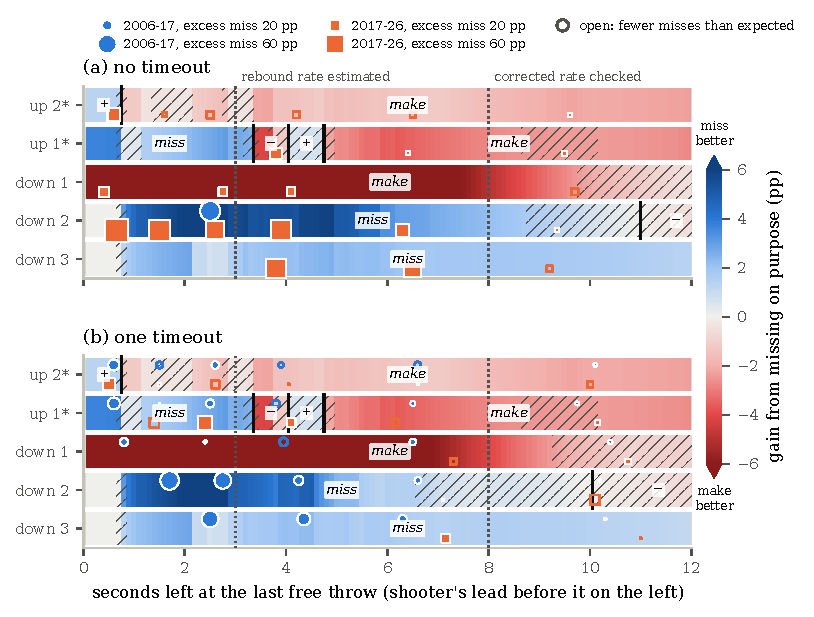
\includegraphics[width=\textwidth]{../figures/fig5_ft_map.pdf}
\caption{Decision map for the last free throw: gain (percentage points) from missing on purpose, by seconds
left and the shooter's lead before the free throw, when the shooting team has no timeout (a) or one (b); the
opponent has none and neither team has a foul to give. Blue and ``miss'': miss; red and ``make'': make; hatched: the 90\% band
includes zero; black lines: decision boundary (as in Figure~\ref{fig:foulmap}); $^\ast$: leading rows, where the
deliberate-miss rebound rate of trailing shooters is extrapolated; dotted lines: the rebound rate is estimated at
most 3 seconds before the end, and the corrected rate is checked up to 8 seconds; $+$/$-$: miss/make on runs shorter than 1.5 seconds; the colour scale saturates at
$\pm 6$. Dots: excess miss rate (observed minus the rate expected from the shooters' free-throw percentages;
filled positive, open negative, area proportional), circles 2006-07 to 2016-17 (blue), squares 2017-18 to
2025-26 (orange), pooled over the opponent's timeouts; cells with fewer than 8 trips are omitted (counts in
\texttt{results/obs\_ft.csv}).}
\label{fig:ftmap}
\end{figure}

Figure~\ref{fig:breakeven} draws the break-even rate \eqref{eq:rstar} against time. Trailing by two
without a timeout, $\rho^{\ast}$ is 0.13 at 3.5 seconds, 0.17 at 5, 0.33 at 8 and 0.47 at 12; the raw
deliberate-miss rebound rate, 0.44 (0.35--0.53), exceeds it up to about 11 seconds, and its lower bound up to about
8.5 seconds, while the rate of 0.13 used by the hand-set model exceeds it only below about 3.8 seconds (and
between 4.3 and 4.9). Descriptively, observed behaviour moved in the direction of the map: trailing by two with at most 5 seconds left, the last free
throw was missed in 54.3\% of trips in 2006-07 to 2016-17 (expected from free-throw percentages 21.8\%, $n=81$)
and in 77.9\% from 2017-18 (expected 19.0\%, $n=95$). Over the same eras the share of trailing teams' phases
without a timeout rose from 5.3\% to 24.0\%.

\begin{figure}[tbp]
\centering
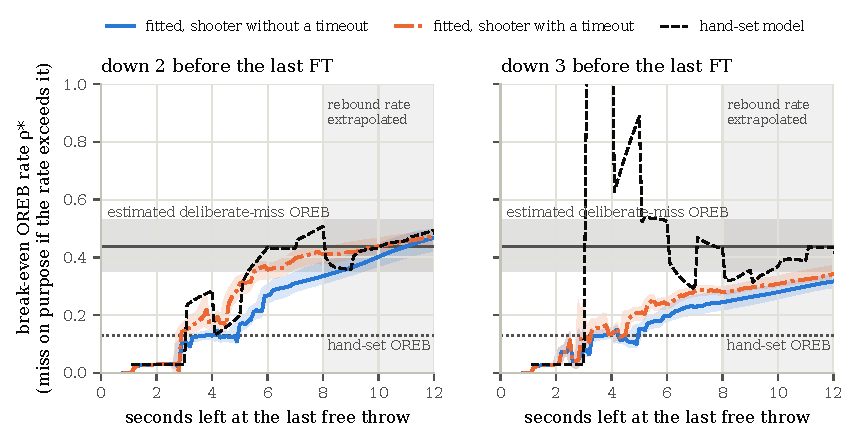
\includegraphics[width=\textwidth]{../figures/fig6_breakeven.pdf}
\caption{Break-even offensive-rebound rate $\rho^{\ast}$ of the deliberate miss \eqref{eq:rstar}: missing on
purpose is optimal when the rebound rate exceeds the curve. Grey band: estimated deliberate-miss rate with
95\% interval; dotted: the hand-set rate; bands on the curves: 90\% bootstrap intervals. The comparison holds the
continuation values fixed (Section~\ref{sec:model}); $\rho^{\ast}$ outside $[0,1]$ or undefined is clipped (ticks at
the frame).}
\label{fig:breakeven}
\end{figure}

\subsection{What the estimated inputs change}

Figure~\ref{fig:gap} (Appendix~\ref{app:figs}) solves the same game with the hand-set inputs. The hand-set model says that the leader
up three gains 11--14 percentage points by fouling with 3--5 seconds left; with estimated inputs the gain lies
between $-2.2$ and $+2.1$, depending on how the trailer inbounds. The difference comes mainly from the rushed
three: the hand-set model gives a team with 4 seconds a 26\% three, the data 7\% from the backcourt. For the free
throw, the hand-set game favours the miss only between 1.1 and 3.0 seconds, the estimated game from 0.8 to
about 11 seconds, because of the deliberate-miss rebound rate. Finally, the value of holding a timeout is
concentrated in the last 4 seconds: 13.6 percentage points for a team down one at about 3 seconds, 8.9 down two,
7.2 tied, and at most 2 beyond 10 seconds (Appendix~\ref{app:figs}, Figure~\ref{fig:advance}).

%% ============================================================================
\section{Model checks and reproducibility} \label{sec:checks}

\emph{Exact verification.} An independent implementation of the Bellman equations in
\proglang{Mathematica}, written from the model specification as a memoised recursion over exact rational
numbers, re-solves a 14-step instance with the fitted shot inputs and small integer durations, chosen so that
every branch is exercised (a 9-step shot clock after offensive rebounds, a 2-step timeout, a 2-step rebound delay
for ordinary free-throw misses and a distribution over 1 and 2 steps for deliberate ones, dead-ball rebound shares, and
$\beta=0.15$). It agrees with the compiled solver on all 3{,}888 values compared (all six start types and both teams'
timeouts and fouls to give at 7 and 14 steps, leads $-4$ to 4) and all 324 free-throw values, to $3.3\times10^{-16}$. The identity \eqref{eq:rstar} holds symbolically for
free symbols, and its sign agrees with the solver on all 90 fitted states checked (Appendix~\ref{app:check}).
Both implementations follow the same written rules, so their agreement checks the numerics, not the rules; unit
tests check the shot-clock transitions separately.

\emph{Invariants.} Unit tests check the rule encoding (timeouts, fouls to give, the shot-clock limits and
targets after a timeout and a side-out) and that, in the solved game, the outcome
probabilities sum to one, values lie in $[0,1]$, values are monotone in the lead and in timeouts held (every start
type), and the defence's foul option never raises the offence's value (every start type except \BC, where the
offence's timeout follows the defence's choice); other tests check each new transition against its formula. A script checks the figure palette under simulated
protanopia, deuteranopia and tritanopia \citep{Machado2009}: the smallest distance between
colours that must be told apart is 9.1 OKLab units (\path{results/palette_check.txt}).

\emph{Calibration.} For the 18{,}372 fourth-period phases from 2006-07 on with at most 24 seconds left and a
lead between $-3$ and 3, the squared error of the model's win probability for the team with the ball (the outcome
counts overtime as $\frac12$) is 0.062, against 0.195 for a constant and 0.061 for an in-sample table of outcomes
by lead and 3-second bin (Appendix~\ref{app:figs}, Figure~\ref{fig:calib}). Out of sample the two have similar squared error: with
all inputs estimated on even seasons and scored on odd seasons, and vice versa, the model scores 0.058 and 0.066
against 0.058 and 0.065 for a table built on the training seasons. The model therefore predicts about as well as
a lookup table, not better; its purpose is the counterfactual comparison of actions, which a table cannot
provide, and good calibration under observed play cannot validate every action contrast. Pooled over eras it
overrates the team with the ball by about 2 percentage points (0.564 predicted, 0.542 observed); candidate causes
are the optimal-play assumption and the single pressure shift of the shot curves.

\emph{Identification.} The curves read the time available as the time a team chooses to use. Shots taken with
time to spare (at least 4 seconds left in the period) are made far more often than forced shots (at most 1 second
left) after the same time used: by 15--54 percentage points for twos (every cell) and by up to 35 for threes (the
interval is above zero in 11 of 15 cells; Appendix~\ref{app:figs}, Table~\ref{tab:ident}). Early shots are therefore taken when a good one appears, and
the time used is not exogenous. The main curves, in time available, average over this choice. Two alternative
specifications, which keep the attempt probability in the time available and are not bounds on the effect of an
instruction to shoot at a given time, refit the success rates on forced shots only (the time used is then the time
available) and in the time used for all shots (as if every early shot were as good as the observed ones). The
recommendations are therefore conditional on the assumed timing model.

\emph{Sensitivity.} Table~\ref{tab:sens} and Figure~\ref{fig:sens} (Appendix~\ref{app:figs}) re-solve the game under
27 variants, each changing one assumption: rebound rates, team-rebound shares and delays (including the empirical
delay distributions of the proxy and of ordinary misses, which are not selected by the clock, and the previous
treatment of team rebounds), foul times, $\beta$, two-point thresholds, the shot clock, the shot curves (score-neutral
and the two identification specifications), the three-shot-foul risk, and inputs re-estimated on either era alone.
Fouling up three after the trailer's timeout gains between 0.1 and 4.8 percentage points at 3 seconds in every
variant (1.2 and 2.4 under the identification specifications, 2.6 and 3.4 with the two delay distributions, 0.1 with
inputs from 2017-18 on); from a backcourt inbound the sign varies ($-2.8$ to $+1.9$). Missing the last free throw
down two gains 3.9 to 8.2 percentage points at 2 seconds and stays positive at 5 seconds in every variant except the
one in which a deliberate miss is rebounded no more often than an accidental one (1.8 points at 2 seconds, nothing
beyond about 5). The maximum value of a timeout (down one) is 13.1--14.2 points except under the time-used curves
(24.1), which credit the frontcourt inbound with selected early shots. One-at-a-time variants do not establish joint
robustness. The foul times may include deliberate waiting, which the shorter-foul variant covers in part.

\emph{Reproducibility.} The data are downloaded from a pinned upstream commit and checked against a committed
checksum manifest. On one platform (macOS), a clean copy of the repository (\code{make env}, \code{make all}) rebuilds
every table, estimate and map with identical numbers in a few minutes plus the bootstrap, and regenerates all
figures; the \proglang{Mathematica} check (\code{make check}) and the platform comparison have their own commands.
The bootstrap ran on a Linux cluster whose environment differs slightly from the lock file (recorded in
\path{results/platform/worker_environment.txt}); three replicates recomputed on macOS (0, 517, 999) agree numerically
with the cluster's, which are deposited in \path{results/platform/reference/}, to $4.7\times10^{-13}$
(\code{scripts/compare_platform.py}), and every replicate stores a
fingerprint of the code and input data that produced it, which the summary checks before use. This comparison
caught a defect during development (rank-deficient spline fits that silently failed to converge); the pipeline now
stops when any fit fails to converge.

%% ============================================================================
\section{Discussion} \label{sec:discussion}

The pipeline turns a public event log into an exact decision model whose probabilities and durations are estimated and
whose uncertainty reaches the final graphic. Three lessons are general. First, hand-set inputs can reverse
decisions: in our comparison the rushed three and the deliberate-miss rebound, both hard to guess, change the
sign of the answers. Second, a decision map with marked uncertainty and behaviour overlaid answers the practical
questions (what to do, how much it matters, how sure we are, what teams do) in one panel. Third, closed-form
break-even quantities such as $\rho^{\ast}$ make a conclusion portable: a reader with a different belief about an
input can read off the decision locally.

The analysis has limits. The deliberate-miss rebound rate rests on 121 misses identified by a proxy; under the
assumptions of Section~\ref{sec:estimation} the raw rate is a lower bound, and the corrected rate is compatible with
a constant rate up to 8 seconds, but beyond 8 seconds it is extrapolated,
which Figures~\ref{fig:ftmap} and \ref{fig:breakeven} mark. The shot curves rest on the assumption that a chosen
shot after $u$ seconds is as good as a forced one, which the data contradict for early shots; two alternative
specifications leave the headline signs unchanged but are not bounds. The curves borrow their shape from score-neutral quarters with a
single pressure shift and use a 0/1 rule for two-point shots that creates kinks in some curves. The defence commits
to a foul of fixed duration, and how often the offence beats it is not identified; within the timing model even
$\beta=1$ leaves the recommendation unchanged, but real offences facing an attempted foul may get better or worse shots
than the fitted ones. The deliberate-miss rate of trailing shooters is applied to leaders without a check. The modern timeout rule's reference to mandatory timeouts is not modelled, which
affects only the timeout-stratified overlays and the calibration. The model predicts no better than a lookup
table. The observed behaviour is descriptive, and we draw no causal conclusion from the overlays. The same
pipeline applies to other leagues with play-by-play data and to other discrete end-game choices, such as the
timing of the last shot.

%% ============================================================================
\section*{Computational details}

The results were obtained with \proglang{Python}~3.13 \citep{python} and the packages \pkg{NumPy}~2
\citep{numpy}, \pkg{pandas}~3 \citep{pandas}, \pkg{statsmodels}~0.15 \citep{statsmodels},
\pkg{Numba}~0.68 \citep{numba} and \pkg{Matplotlib}~3 \citep{matplotlib}; exact versions are pinned in
\code{requirements-lock.txt}. The symbolic checks used \proglang{Mathematica}~15.0.0 for Mac~OS~X ARM
\citep{mathematica}. The bootstrap ran on a computing cluster (Rocky Linux 9.2), everything else on a laptop.
Code, derived results, the figures and the scripts that download the data are available at
\url{https://github.com/HeirOfIsildur/nba-endgame-jdssv}; the play-by-play data are downloaded from
\url{https://github.com/shufinskiy/nba_data} at a pinned commit and verified against a committed checksum manifest.

\section*{Acknowledgments}

The research of Jan Janou\v{s}ek and Michal Pe\v{s}ta was supported by the Czech Science
Foundation project GA\v{C}R No.~27-25747L and by the Charles University Grant Agency project
GA~UK No.~188325.

\section*{Declaration of generative AI and AI-assisted technologies}

During the preparation of this work the authors used large language models (Anthropic's Claude and OpenAI's GPT
models) to improve the English of the manuscript, as non-native speakers; to check derivations, formulas and
arithmetic; and to assist in writing and reviewing the analysis code. After using these tools, the authors reviewed and
edited the content as needed and take full responsibility for the content of the publication.

\bibliography{refs}

%% ============================================================================
\newpage
\begin{appendix}

\section{Exact verification in Mathematica} \label{app:check}

The \proglang{Mathematica} script \path{checks/dp_check.wl} (in the supplement) re-solves a small instance of the game
independently of the \proglang{Python} solver: 14 time steps, shot inputs rounded to exact thousandths of the fitted
inputs and durations rounded to small integers (\path{checks/dp_small_inputs.json}). It defines the value function
directly from \eqref{eq:W}, \eqref{eq:V} and \eqref{eq:F} as a memoised recursion over exact rational numbers, with
the same shot-clock and rebound rules as the solver. Because the recursion follows the dependencies itself, it does
not share the solver's loop order, which is part of what it checks. The maximum absolute difference from the solver
is $3.3\times10^{-16}$ over 3{,}888 values of $V$ and $2.4\times10^{-16}$ over 324 free-throw values. The
break-even identity \eqref{eq:rstar} is proved with \code{FullSimplify} on free symbols, and on 90 fitted states its
residual is $1.4\times10^{-16}$ with matching signs. All checks pass with \proglang{Mathematica} 15.0.0
(\path{checks/dp_check_out.json}).

\section{Additional figures and tables} \label{app:figs}

\begin{table}[h!]
\centering
\caption{Identification check: field-goal percentage of shots taken with time to spare (at least 4 seconds left in
the period, so the time available exceeds the time used by at least 4 seconds) minus that of forced shots (at most
1 second left), in percentage points, by shot value, start type and seconds used, all curve-sample phases; 90\%
game-bootstrap intervals; --: fewer than 20 shots in a group (\texttt{results/ident\_check.csv}).}
\label{tab:ident}
\footnotesize\setlength{\tabcolsep}{4pt}
\begin{tabular}{llcccc}
\toprule
$k$ & Start & 0.5--2 s & 2--4 s & 4--6 s & 6--10 s \\
\midrule
3 & backcourt inbound & -- & +20 (+9, +33) & +15 (+7, +22) & +7 (+2, +12) \\
3 & frontcourt after timeout & +6 ($-$1, +14) & +10 (+4, +15) & +9 (+3, +16) & +7 (+0, +15) \\
3 & live ball & +35 (+23, +47) & +26 (+21, +32) & +18 (+13, +22) & +11 (+6, +15) \\
3 & offensive rebound & +22 (+17, +28) & +8 (+2, +14) & +8 ($-$2, +18) & $-$6 ($-$19, +6) \\
2 & backcourt inbound & -- & +26 (+16, +35) & +25 (+19, +31) & +19 (+15, +24) \\
2 & frontcourt after timeout & +54 (+40, +67) & +31 (+24, +39) & +26 (+19, +33) & +21 (+15, +28) \\
2 & live ball & +54 (+50, +58) & +38 (+36, +41) & +28 (+25, +31) & +17 (+13, +21) \\
2 & offensive rebound & +15 (+12, +17) & +15 (+10, +20) & +20 (+10, +30) & +15 (+3, +26) \\
\bottomrule
\end{tabular}

\end{table}

\begin{figure}[h!]
\centering
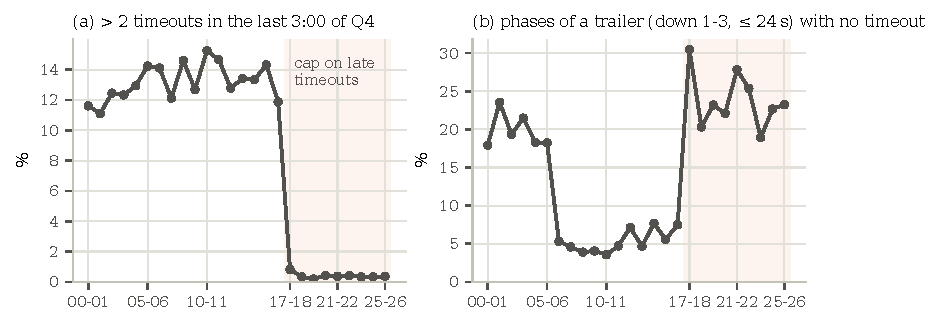
\includegraphics[width=\textwidth]{../figures/fig1_timeouts.pdf}
\caption{The 2017-18 cap on late timeouts in the data. (a) Share of team-games with more than two timeouts
in the last 3:00 of the fourth period. (b) Share of trailing teams (down 1--3, at most 24 seconds left) with
no timeout left. Seasons are labelled 00-01 for 2000-01 and so on; the shaded area is the capped era.}
\label{fig:timeouts}
\end{figure}

\emph{Deliberate-miss proxy audit} (\code{linkage.py}). The event after each of the 131 proxy misses is a defensive
rebound in 46, a live offensive rebound in 40, a team rebound (a dead ball out of bounds) to the opponent in 22 and to
the shooting team in 15, the end of the period in 4 and a tip or a violation before any logged rebound in 4. In 118 of
the 121 retained misses the rebound linked to the free throw is the first event after it, a median 0.6 seconds later
(5\% after more than 2 seconds); without the three ambiguous links the rate is 0.43. It is 0.42 before 2017-18 and
0.47 after.

\begin{table}[p]
\centering
\caption{Sensitivity variants (\texttt{results/sensitivity.csv}; the table is generated by \texttt{headline.py}): gain in
percentage points from fouling up three at 3 seconds (after the trailer's last timeout, \FC, or from a backcourt
inbound, \BC) and from missing the last free throw down two at 2 and 5 seconds (no timeouts), the last time at which
that gain is at least 1 point, and the largest value of a timeout for a team down one.}
\label{tab:sens}
\scriptsize
\begin{tabular}{p{7.4cm}rrrrrr}
\toprule
Variant & \multicolumn{2}{c}{Foul up 3, 3 s} & \multicolumn{2}{c}{Miss down 2} & $\ge$1 pp & Timeout \\
 & \FC & \BC & 2 s & 5 s & until (s) & max \\
\midrule
main estimate & +1.8 & $-$1.4 & +6.0 & +5.1 & 9.7 & 13.6 \\
deliberate-miss OREB at its lower 95\% bound (0.35) & +2.8 & $-$0.7 & +4.7 & +3.3 & 6.4 & 13.6 \\
deliberate-miss OREB mixture-corrected (0.55) & +0.6 & $-$2.3 & +7.7 & +7.9 & 18.7 & 13.6 \\
deliberate-miss OREB = ordinary (0.15) & +4.8 & +0.8 & +1.8 & $-$0.4 & 2.8 & 13.6 \\
fouls take 0.5 s longer & +3.7 & +1.9 & +6.0 & +5.7 & 10.1 & 13.6 \\
fouls take 0.5 s less & +1.5 & $-$2.8 & +6.0 & +4.2 & 9.2 & 13.6 \\
offence beats a committed foul with probability 0.1 & +1.8 & $-$1.4 & +6.0 & +5.1 & 9.7 & 13.6 \\
offence beats a committed foul with probability 0.2 & +1.8 & $-$1.4 & +6.0 & +5.1 & 9.7 & 13.6 \\
offence always beats a committed foul (probability 1, an extreme) & +1.8 & $-$1.4 & +6.0 & +5.2 & 9.7 & 13.6 \\
two-point threshold 15\% & +1.8 & $-$1.4 & +6.0 & +3.8 & 9.7 & 13.6 \\
two-point threshold 35\% & +1.8 & $-$1.4 & +6.0 & +5.1 & 9.7 & 13.6 \\
no shot-clock reset after OREB & +1.8 & $-$1.4 & +6.0 & +5.1 & 9.7 & 13.6 \\
score-neutral shot curves (no pressure shift) & +1.1 & $-$1.3 & +7.0 & +6.2 & 9.0 & 13.1 \\
3-FT risk at its lower bound (0.06) & +2.4 & $-$0.9 & +6.0 & +5.1 & 9.7 & 13.6 \\
3-FT risk at its upper bound (0.11) & +1.2 & $-$2.0 & +6.0 & +5.2 & 9.7 & 13.6 \\
OREB on missed FG at 0.40 & +1.8 & $-$1.4 & +6.0 & +5.1 & 9.7 & 13.6 \\
deliberate-miss OREB: live rebounds only (0.34) & +2.5 & $-$1.0 & +4.9 & +3.1 & 6.1 & 13.6 \\
FT team rebounds (both teams) as live rebounds & +1.3 & $-$1.8 & +6.4 & +5.2 & 9.8 & 13.6 \\
deliberate-miss OREB from down-3 trips only (0.29) & +3.3 & $-$0.3 & +3.9 & +2.2 & 5.8 & 13.6 \\
one FT rebound time for all misses, the deliberate one (0.69 s) & +1.8 & $-$1.4 & +6.0 & +4.9 & 9.6 & 13.6 \\
one FT rebound time for all misses, the ordinary one (1.08 s) & +3.0 & +1.9 & +5.5 & +5.8 & 9.5 & 13.6 \\
rebound curves include team-rebound starts; FG team rebounds live (previous treatment) & +3.1 & $-$0.2 & +5.3 & +4.9 & 9.6 & 13.5 \\
deliberate-miss FT rebound delay: empirical distribution of the proxy & +2.6 & $-$0.8 & +5.6 & +4.7 & 9.6 & 13.6 \\
deliberate-miss FT rebound delay: distribution of ordinary misses (not clock-selected) & +3.4 & $-$0.1 & +4.7 & +4.8 & 9.4 & 13.6 \\
FG\% from forced shots only (identification) & +1.2 & $-$1.5 & +5.5 & +5.0 & 10.8 & 14.2 \\
FG\% by time used, all shots (identification) & +2.4 & $-$2.8 & +7.6 & +6.4 & 7.8 & 24.1 \\
all inputs from 2000-01 to 2016-17 only & +2.3 & $-$0.8 & +5.4 & +4.7 & 9.0 & 13.9 \\
all inputs from 2017-18 to 2025-26 only & +0.1 & +1.2 & +8.2 & +7.2 & 10.6 & 13.3 \\
\bottomrule
\end{tabular}

\end{table}

\begin{figure}[h!]
\centering
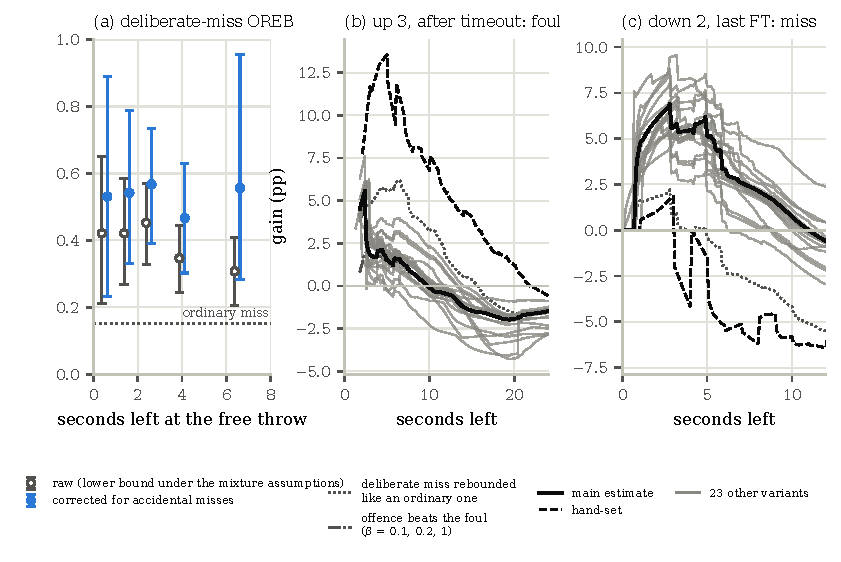
\includegraphics[width=\textwidth]{../figures/fig10_sensitivity.pdf}
\caption{(a) Deliberate-miss offensive-rebound rate by time window (shooter down 2--3): raw share of misses
rebounded (a lower bound under the mixture assumptions of Section~\ref{sec:estimation}) and the rate corrected for accidental misses, with 95\% game-bootstrap intervals;
dotted: the rate after an ordinary miss. (b, c) The two headline curves under the 27 sensitivity variants of Table~\ref{tab:sens} (grey; dash-dot:
the offence beats the foul with probability $\beta$), with the main estimate (black) and the hand-set model (dashed).}
\label{fig:sens}
\end{figure}

\begin{figure}[h!]
\centering
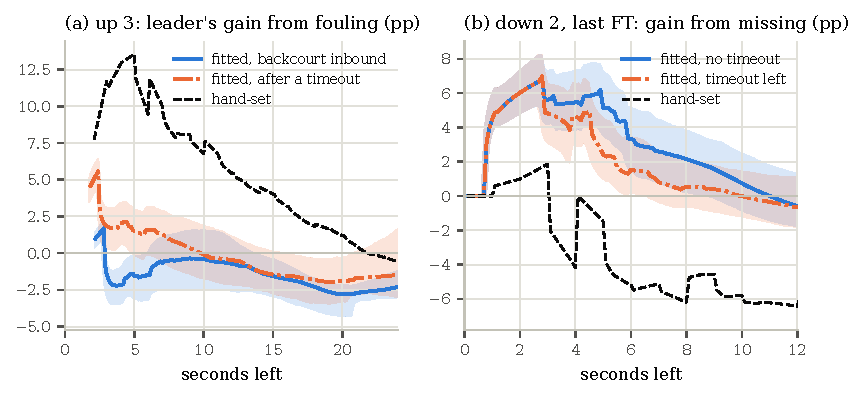
\includegraphics[width=\textwidth]{../figures/fig7_hand_vs_fitted.pdf}
\caption{Hand-set inputs (dashed) against estimated inputs (lines with 90\% bootstrap bands) in the same
game: (a) leader's gain from fouling up three; (b) gain from missing the last free throw when trailing by
two.}
\label{fig:gap}
\end{figure}

\begin{figure}[h!]
\centering
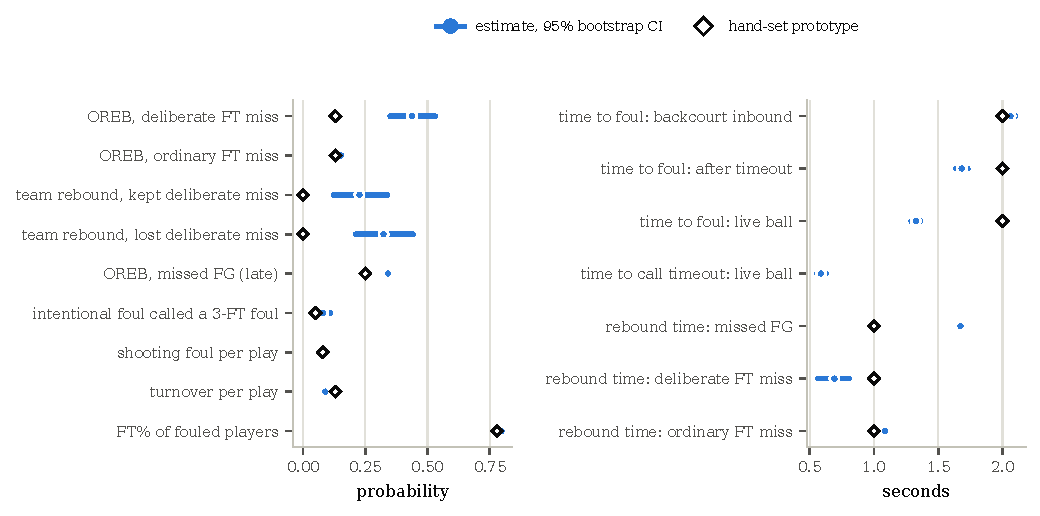
\includegraphics[width=\textwidth]{../figures/fig3_inputs.pdf}
\caption{Scalar inputs: estimates with 95\% bootstrap intervals (blue) and hand-set values (diamonds).}
\label{fig:inputs}
\end{figure}

\begin{figure}[h!]
\centering
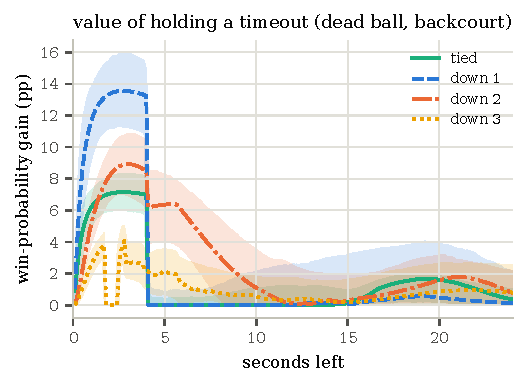
\includegraphics[width=0.62\textwidth]{../figures/fig9_advance.pdf}
\caption{Value of holding one timeout (the option to stop the clock and inbound in the frontcourt) for a
team inbounding a dead ball in the backcourt, by deficit and seconds left, with 90\% bootstrap bands; the opponent
has no timeout and neither team has a foul to give.}
\label{fig:advance}
\end{figure}

\begin{figure}[h!]
\centering
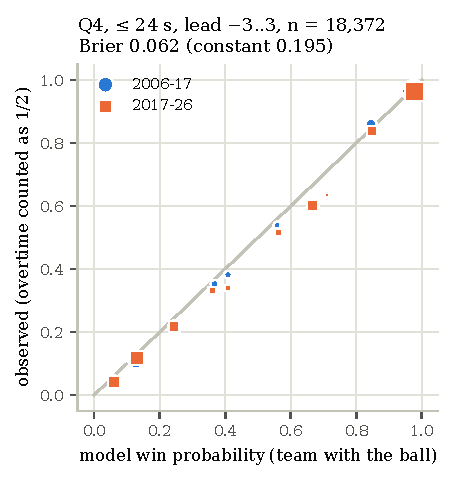
\includegraphics[width=0.5\textwidth]{../figures/fig8_calibration.pdf}
\caption{Calibration: model win probability of the team with the ball against the observed result
(overtime counted as $\frac12$), fourth-period phases with at most 24 seconds left and a lead between $-3$
and 3, by era; point area proportional to the number of phases.}
\label{fig:calib}
\end{figure}

\clearpage
\end{appendix}

\end{document}
